\documentclass[11pt,a4paper]{article}

% Packages
\usepackage[utf8]{inputenc}
\usepackage[spanish, es-tabla, es-lcroman]{babel}
\usepackage{caption}
\usepackage{listings}
\usepackage{adjustbox}
\usepackage[shortlabels]{enumitem}
\usepackage{boldline}
\usepackage{amssymb, amsmath}
\usepackage[margin=1in]{geometry}
\usepackage{xcolor, color}
\usepackage{soul}
\usepackage{epstopdf}

% Meta
\title{\textbf{ESTRUCTURA DE DATOS}\\
	   \textit{Práctica 1. Eficiencia de algoritmos}\\
	   \large \vspace{0.25em} Doble Grado de Informática y Matemáticas}
\author{José María Martín Luque\\ Antonio Coín Castro}
\date{\today}

% Custom
\providecommand{\abs}[1]{\lvert#1\rvert}
\setlength\parindent{0pt}
\definecolor{Light}{gray}{.90}
\definecolor{mygreen}{rgb}{0,0.6,0}
\definecolor{mygray}{rgb}{0.5,0.5,0.5}
\definecolor{mymauve}{rgb}{0.58,0,0.82}
\renewcommand\labelenumi{(\emph{\roman{enumi})}}
\newcommand{\bm}[1]{\boldsymbol{#1}}

\lstset{literate=   % listings config
  {á}{{\'a}}1 {é}{{\'e}}1 {í}{{\'i}}1 {ó}{{\'o}}1 {ú}{{\'u}}1
  {Á}{{\'A}}1 {É}{{\'E}}1 {Í}{{\'I}}1 {Ó}{{\'O}}1 {Ú}{{\'U}}1
  {à}{{\`a}}1 {è}{{\`e}}1 {ì}{{\`i}}1 {ò}{{\`o}}1 {ù}{{\`u}}1
  {À}{{\`A}}1 {È}{{\'E}}1 {Ì}{{\`I}}1 {Ò}{{\`O}}1 {Ù}{{\`U}}1
  {ä}{{\"a}}1 {ë}{{\"e}}1 {ï}{{\"i}}1 {ö}{{\"o}}1 {ü}{{\"u}}1
  {Ä}{{\"A}}1 {Ë}{{\"E}}1 {Ï}{{\"I}}1 {Ö}{{\"O}}1 {Ü}{{\"U}}1
  {â}{{\^a}}1 {ê}{{\^e}}1 {î}{{\^i}}1 {ô}{{\^o}}1 {û}{{\^u}}1
  {Â}{{\^A}}1 {Ê}{{\^E}}1 {Î}{{\^I}}1 {Ô}{{\^O}}1 {Û}{{\^U}}1
  {œ}{{\oe}}1 {Œ}{{\OE}}1 {æ}{{\ae}}1 {Æ}{{\AE}}1 {ß}{{\ss}}1
  {ű}{{\H{u}}}1 {Ű}{{\H{U}}}1 {ő}{{\H{o}}}1 {Ő}{{\H{O}}}1
  {ç}{{\c c}}1 {Ç}{{\c C}}1 {ø}{{\o}}1 {å}{{\r a}}1 {Å}{{\r A}}1
  {€}{{\EUR}}1 {£}{{\pounds}}1 {ñ}{{\~{n}}}1
}

\lstset{    %listings config
  language=C++,
  belowcaptionskip=1\baselineskip,
  breaklines=true,
  frame=L,
  xleftmargin=0.5in,
  %otherkeywords={},
  showstringspaces=false,
  backgroundcolor=\color{white},
  basicstyle=\footnotesize\ttfamily,
  keywordstyle=\bfseries\color{purple!90!black},
  commentstyle=\itshape\color{gray!85!},
  identifierstyle=\color{blue!80!black},
  stringstyle=\color{green!60!black},
}

\newcommand\ddfrac[2]{\frac{\displaystyle #1}{\displaystyle #2}}

% Environments

\begin{document}
\maketitle

\section*{Ejercicio 1.}
En este ejercicio, comprobaremos tanto la eficiencia teórica como la eficiencia empírica del algoritmo de ordenación \emph{burbuja}:

\begin{lstlisting}[numbers=left]
void ordenar_burbuja(int *v, int n)
{
  for (int i=0; i<n-1; i++)
    for (int j=0; j<n-i-1; j++)
      if (v[j]>v[j+1]) {
        int aux = v[j];
        v[j] = v[j+1];
        v[j+1] = aux;
      }
}
\end{lstlisting}

Comencemos analizando la eficiencia teórica del algoritmo, en el caso peor. Veamos primero el coste en operaciones elementales (OE) de cada línea:\\

\textbf{Línea 3.} Hay 5 OE: una asignación, una resta, una comparación y un incremento(incremento + asignación).

\textbf{Línea 4.} Hay 6 OE: igual que la línea anterior, pero se realizan dos restas.

\textbf{Línea 5.} Hay 4 OE: dos accesos a un vector, una suma y una comparación.

\textbf{Línea 6.} Hay 2 OE: asignación y acceso al vector.

\textbf{Línea 7.} Hay 4 OE: dos accesos, suma y asignación.

\textbf{Línea 8.} Hay 3 OE: acceso, suma y asignación.\\

Entonces, la eficiencia del algoritmo es:

$$ T(n) = \sum_{i=0}^{n-2} \left( 5 + \sum_{j=0}^{n-i-2} 19 \right) = \sum_{i=0}^{n-2} \left( 5 + 19(n-i-1) \right) = \sum_{i=0}^{n-2} 19n\ - \sum_{i=0}^{n-2} 19i\ - \sum_{i=0}^{n-2} 14 = $$ $$ = 19n(n-1) - 19 \left( \frac{0 + (n-2)}{2} \cdot (n-1) \right) - 14(n-1) = \frac{19}{2}n^2 - \frac{9}{2} n - 5$$.

Por tanto, afirmamos que $T(n) \in O(n^2)$, y el algoritmo de ordenación burbuja es de orden de eficiencia $O(n^2)$.\\

Ahora creamos un programa de prueba para analizar la eficiencia empírica, haciendo uso de la biblioteca \emph{ctime} del lenguaje C++:

\lstinputlisting{burbuja.cpp}

Al analizar la eficiencia empírica del algoritmo, obtenemos la siguiente gráfica:\\

\begin{center}
	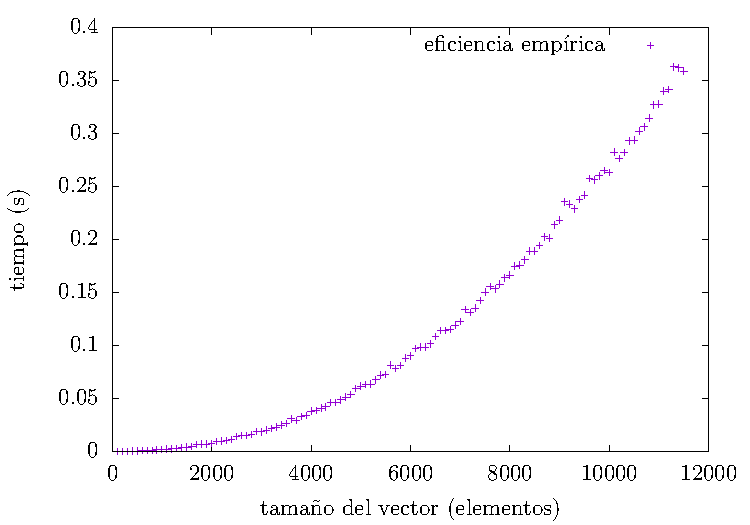
\includegraphics{img/tiempos_ordenacion.pdf}
\end{center}
%%% gráfica eficiencia empírica

Si representamos superpuestas la función de la eficiencia teórica y la empírica, obtenemos lo siguiente:\\

\begin{center}
	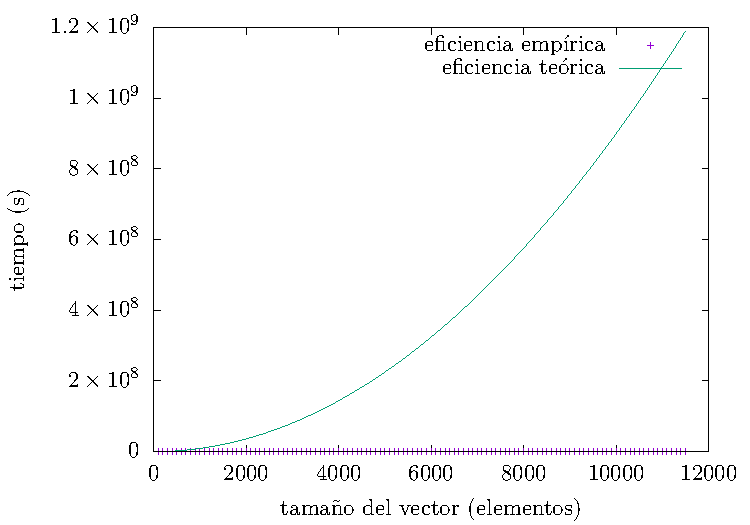
\includegraphics{img/tiempos_ordenacion_teorica_superpuesta.pdf}
\end{center}

%%% gráfica superpuesta

Observamos que %%%conclusión (depende de lo que salga)

\section*{Ejercicio 2.}
Veamos que podemos ajustar, mediante \textit{gnuplot}, los puntos obtenidos al analizar la eficiencia teórica en una función de la forma $f(n) = an^2 + bn + c$.\\

En efecto, obtenemos que la función en cuestión es: $\bm{f(n) = n^2 + n + }$, y la representación gráfica es la siguiente:    %%% función ajustada

\begin{center}
	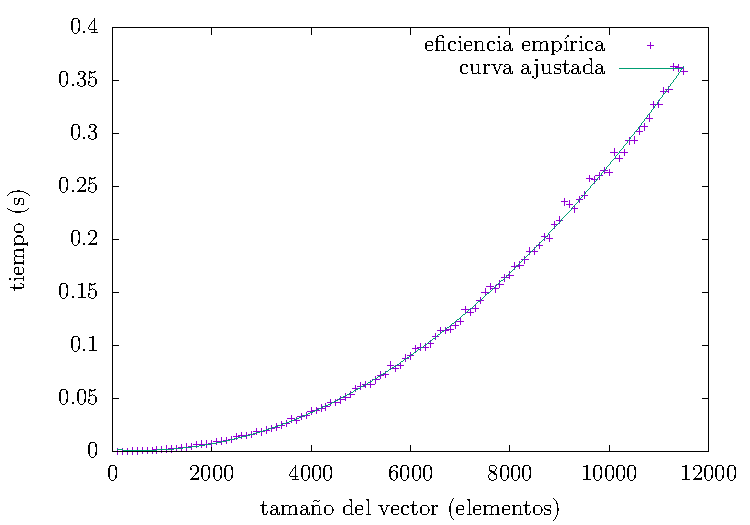
\includegraphics{img/tiempos_ordenacion_ajustado.pdf}
\end{center}

\section*{Ejercicio 3.}

\textbf{a)} En este primer apartado, describiremos el funcionamiento del algoritmo proporcionado en el archivo $ejercicio\_desc.cpp$.\\

Se trata de un algoritmo de \textbf{búsqueda binaria}, donde dado un vector $v$ de $n$ elementos enteros, busca el entero $x$ en él. Para ello, se pasan como parámetros el inicio \textit{(inf)} y el final (\textit{sup}) de dicho vector. La función devuelve la posición donde se ha encontrado el elemento, o $-1$ si no estaba en el vector.\\

Para el correcto funcionamiento del algoritmo, es imprescindible que el vector esté \textbf{ordenado}, pues el procedimiento es el siguiente:

\begin{enumerate}
\item Se establece la posición $med = (inf+sup)/2$.
\item Se comprueba si el elemento $x$ está en la posición $med$.
\item Si está, hemos acabado. Si no está, se comprueba si el elemento $v[med]$ es mayor o menor que $x$.
    \begin{itemize}
    \item Si $v[med] < x$, actualizamos $inf = med + 1$
    \item Si $v[med] > x$, actualizamos $sup = med - 1$
    \end{itemize}
\item Repetimos el proceso, hasta encontrar el elemento, o concluir que no está en el vector.
\end{enumerate}

En resumen, el procedimiento se basa en dividir el vector original por la mitad, y si no está ahí el elemento buscado, nos quedamos únicamente con el sub-vector donde se puede encontrar dicho elemento (recordemos que el vector está ordenado). Repitiendo el proceso, acabaremos encontrando el elemento, o descubriendo que no está en el vector, cuando ya no se puedan hacer más divisiones.\\

\textbf{b)} Para el cálculo de la eficiencia teórica de la \textit{búsqueda binaria}, nos basamos en el hecho de que se divide sucesivamente en dos un vector de tamaño $n$. En el caso peor, el proceso continuará hasta que no se puedan hacer más divisiones del vector.\\

Por definición, el número máximo de veces que se puede dividir por la mitad un vector de tamaño $n$ es $\log_2 (n)$ veces. Para ilustrarlo, consideramos un vector de $n$ elementos. Sabemos que tras $m$ divisiones, el número de elementos restantes será, como mucho, $\left[\frac{n}{2^m}\right]$, y se detendrá cuando dicho número sea menor que 1. Aplicando logaritmos, se tendría que $\log_2 (n) < m$.\\

Como el resto de operaciones son elementales ($O(1)$), concluímos que la eficiencia del algoritmo es logarítmica, es decir, $T(n) \in O(\log (n))$.\\

\textbf{c)} Para analizar la eficiencia empírica, repetimos el proceso de los ejercicios anteriores, obteniendo la siguiente nube de puntos:

\begin{center}
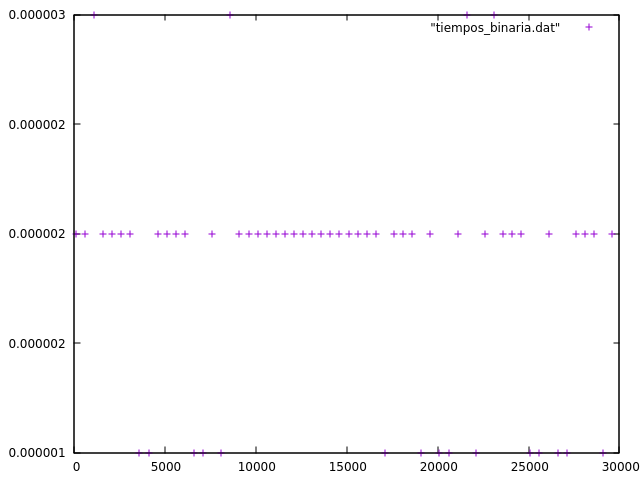
\includegraphics[width=15cm]{img/tiempo_binaria.png}       %%% mejorar gráfica (?)
\end{center}

Vemos que ocurre algo extraño: la eficiencia parece constante. Esto se contradice con nuestro análisis teórico, pero ocurre por dos motivos: el algoritmo se ejecuta tan rápidamente que no es posible medir el tiempo con \textit{ctime}, y la función logaritmo crece lentamente. Para solucionarlo, podemos optar por realizar un número grande de ejecuciones para cada tamaño del vector, y dividir el tiempo total entre el número de ejecuciones.\\

Vemos la gráfica resultante, con $1000$ ejecuciones para cada $n$, y la curva de regresión correspondiente. Ahora sí es bueno el ajuste de la eficiencia empírica a la teórica, mediante la función $\bm{f(n) = }$ %%% parámetros

%%% gráfico puntos + curva regresión

\section*{Ejercicio 4.}

\textbf{a)} Para este apartado, construimos un vector ordenado para representar el caso mejor. Usaremos, por ejemplo, el siguiente código, y elegiremos $vmax > tam$:

\begin{lstlisting}
  // Generación del vector ordenado
  int *v=new int[tam];       // Reserva de memoria
  v[0] = 0;
  for (int i=1; i<tam; i++)  // Recorrer vector
    v[i] = v[i-1] + 1;    // Generar aleatorio [0,vmax[
\end{lstlisting}

La gráfica que representa la eficiencia empírica es la siguiente, cuya función ajustada a la eficiencia teórica es: $\bm{f(n) = }$\\  %%% función ajustada

%%% gráfica


\textbf{b)} Para este apartado, construimos un vector ordenado en orden inverso, para representar el caso peor. Usaremos, el siguiente código:

\begin{lstlisting}
  // Generación del vector ordenado
  int *v=new int[tam];       // Reserva de memoria
  v[0] = vmax;
  for (int i=1; i<tam; i++)  // Recorrer vector
    v[i] = v[i-1] - 1;    // Generar aleatorio [0,vmax[
\end{lstlisting}

La gráfica que representa la eficiencia empírica es la siguiente, cuya función ajustada a la eficiencia teórica es: $\bm{f(n) = }$\\  %%% función ajustada

%%% gráfica

Si comparamos ambas funciones ajustadas con la del \textit{Ejercicio 1}, observamos que el algoritmo es más eficiente en el caso mejor, y menos eficiente en el caso peor, tal y como indicaba la teoría.

\section*{Ejercicio 5.}

Consideramos la siguiente representación alternativa del algoritmo de ordenación \textbf{burbuja}:

\begin{lstlisting}
void ordenar(int *v, int n) {
    bool cambio=true;
    for (int i=0; i<n-1 && cambio; i++) {
        cambio=false;
        for (int j=0; j<n-i-1; j++)
            if (v[j]>v[j+1]) {
            cambio=true;
            int aux = v[j];
            v[j] = v[j+1];
            v[j+1] = aux;
        }
    }
}
\end{lstlisting}

En esta versión, se ha añadido una variable que permite saber si, en una iteración del bucle externo, no se ha producido un cambio en el vector. Si esto ocurre, el vector ya está ordenado, y no hay que continuar.\\

Si realizamos un estudio teórico de la eficiencia en el mejor caso, es decir, cuando el vector de entrada está ya ordenado, nos damos cuenta rápidamente de que el orden de eficiencia es linear, es decir, $T(n) \in O(n)$. Esto es así porque tan sólo habría que recorrer una vez $n-1$ elementos del vector, hasta darse cuenta de que está ordenado.\\

Analicemos ahora la eficiencia empírica de este algoritmo en el caso mejor. Veamos la gráfica asociada:

\begin{center}
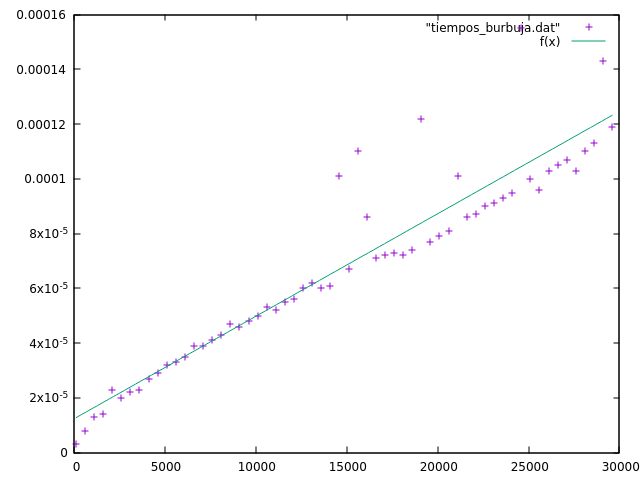
\includegraphics[width=15cm]{img/tiempo_burbuja_modificada}
\end{center}

Como podemos observar, el orden de eficiencia es efectivamente lineal, tal y como había predicho nuestro estudio teórico.

\section*{Ejercicio 6.}
%%% ejercicios voluntarios. ¿Hacer algunos?

\end{document}
